\documentclass[12pt,a4paper]{article}
\usepackage[utf8]{inputenc}
\usepackage[norsk]{babel}
\usepackage{amsmath, amssymb, amsthm}  % For matematisk notasjon
\usepackage{algorithm, algorithmic}    % For å skrive algoritmer
\usepackage{enumitem}
\usepackage{booktabs}
\usepackage{graphicx}                  % For å inkludere bilder
\usepackage{hyperref}                  % For hyperlenker
\usepackage{pgfplots}                  % For grafer
\pgfplotsset{compat=1.16}
\hypersetup{
    colorlinks=false,
    pdfborder={0 0 0},
    }


\title{Øving n - Algoritmer og datastrukturer}
\author{Henrik Halvorsen Kvamme}
\date{\today}

\begin{document}

\begin{center}
    
\includegraphics[width=0.5\textwidth]{../images/NTNU_Logo.png}
    
    \vspace{1.5em}  % Optional vertical space
    
    {\LARGE \textbf{Øving 8} \\[0.5em] \text{Algoritmer og Datastrukturer}}  % Title
    \vspace{1em}  % Optional vertical space
    
    {\large Henrik Halvorsen Kvamme}\\  % Author name
    \vspace{0.5em}  % Optional vertical space
    
    {\today}  % Date
\end{center}

\vspace{2em}

\tableofcontents

\newpage

\section{Introduksjon}
Denne rapporten beskriver utviklingen av et komprimerings- og dekomprimeringsprogram. Komprimering av data er en fundamental operasjon i informasjonsteknologi, som muliggjør effektiv lagring og overføring av data. I denne øvingen anvendes den velkjente komprimeringsteknikken Lempel-Ziv-Welsh (LZW), en videreutvikling av Lempel-Ziv (LZ). Formålet er å implementere disse algoritmene for å redusere størrelsen på filer uten å miste informasjon og deretter nøyaktig gjenopprette originaldataene via dekomprimering. Rapporten vil dekke teoretisk grunnlag, implementasjonsdetaljer, resultatene av komprimeringstester, og diskusjon av programmets effektivitet og anvendelighet.

\section{Teori}
\subsection{Generell komprimeringsteori}
Komprimering av filer er prosessen med å redusere filstørrelsen ved å anvende algoritmer som identifiserer og eliminerer redundans i dataene. To hovedtyper av komprimering er \textbf{lossless} og \textbf{lossy} komprimering. Mens \textit{lossless} komprimering tillater en perfekt gjenopprettelse av originaldata, tillater \textit{lossy} komprimering at noe data går tapt for å oppnå høyere komprimeringsrater. I denne oppgaven fokuserer vi på \textit{lossless} komprimeringsmetoder.

\subsection{Lempel-Ziv-Welsh (LZW)}
LZW er en komprimeringsalgoritme som reduserer filstørrelse ved å erstatte gjentakende data med kortere referanser. Den er populær i filformater som GIF og PDF.

\subsection{Utfordinger med filkomprimering}
Komprimeringsteknikker står overfor flere utfordringer, spesielt når det gjelder å håndtere forskjellige typer data. For eksempel, mens tekstfiler ofte komprimeres effektivt, kan binære filer eller allerede komprimerte filer (som JPEG-bilder) ikke komprimeres like mye og noen ganger kan de øke i størrelse når man prøver å komprimere dem. Derfor er det viktig å forstå datakonteksten og velge riktig komprimeringsalgoritme tilsvarende.

\section{Resultater}
Etter å ha implementert LZW komprimeringsalgoritmen, ble det utført flere tester for å evaluere effektiviteten. Her er et resultat på en av testfilene i oppgaven, 'diverse.txt':
\begin{figure}[h]
    \centering
    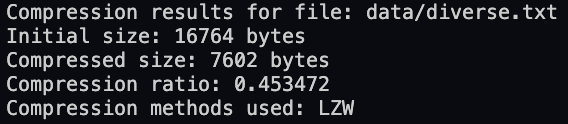
\includegraphics[width=0.8\textwidth]{resultat.png}
    \caption{Bare 45\% av stlørrelsen!}
\end{figure}

\section{Konklusjon}
Jeg valgte å gjøre som de to tidligere oppgavene med å implementere en klasse for å lese in data fra fil. Den tar inn filnavn og bruker fstream for å lese og skrive data. Klassen har metode for å komprimere og dekomprimere filer.

Kildekoden ligger vedlagt i main.cpp. Et nytt objekt for den komprimerte filen blir oprettet for å vise at den ikke overfører tilstand fra da den komprimerte.x

\end{document}